\section{Related software and work}
In this section we will cover Cassandra and HBase. Two other distributed systems with similar applications as Voldemort. We will also cover some related work on automated scaling in Cassandra. 

\subsection{Cassandra}
Cassandra is a scalable NoSQL database now available as open source through the Apache foundation. It was built from scratch with goal of being a massively scalable NoSQL database. In a cluster running Cassandra there is no sense of a master node, and all communication between nodes use peer to peer and the gossip protocol. As an administrator it is easy to scale Cassandra to meet both current and future system requirements. 

\subsubsection{Reads and writes}
In Cassandra all participating nodes can be accessed for writes and reads. To ensure durability all writes are preceded by a write to a commit log. If a node has crashed, a node holding a replica will service reads and writes according to the hinted handoff strategy. As with Voldemort, Cassandra also features tunable consistency. 

\subsubsection{Data model}
The Cassandra data model is based on a key:value model, however Cassandra extends this model with up to two levels of nesting. This forms a map structure called columns where the outer row key acts as a primary key and the inner sorted map holds all information: \texttt{Map<RowKey, SortedMap<ColumnKey, ColumnValue>>}. By using maps we achieve easy lookups and range scans. By adding one more level of nesting we can group columns. These are called super columns. 
In Cassandra de-normalization in important to efficiently perform queries that accesses information stored in separate columns. To allow for faster loopups composite columns can be created to match the need of one or more specific queries. These composite columns simply duplicate information already stored in various columns for easier access. 

\begin{figure}[h]
    \centering
    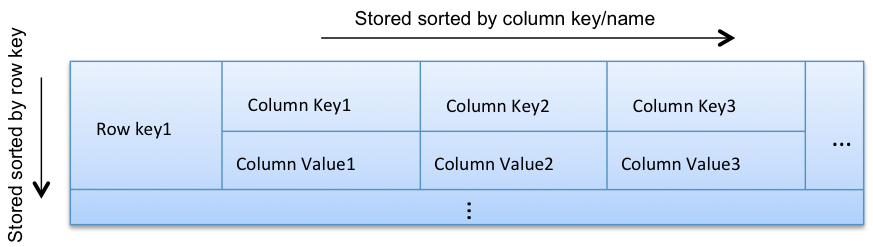
\includegraphics[width=0.5\textwidth]{resources/cas_col.png}
    \caption{A sample Cassanda column. The row key acts as a primary key and each key:value pair would hold one field in a table. Images borrowed from www.ebaytechblog.com}
    \label{fig:sample_col}
\end{figure}

\begin{figure}[h]
    \centering
    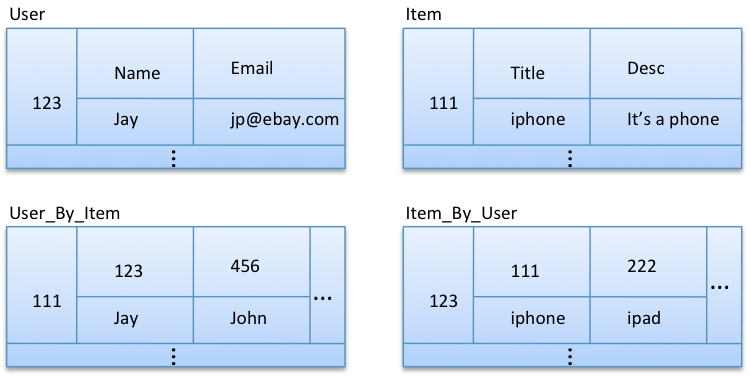
\includegraphics[width=0.6\textwidth]{resources/cas_comp_col.png}
    \caption{A sample Cassandra composite columns. Here we have separate composite column to efficiently be able to serve queries on users by item and item by users.}
    \label{fig:sample_comp_col}
\end{figure}

\begin{figure}[ht]
	\centering
	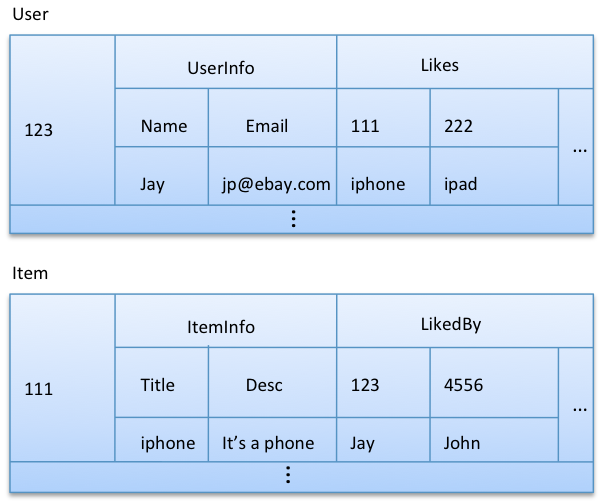
\includegraphics[width=0.4\textwidth]{resources/cas_super_col.png}
	\caption{A sample Cassandra super column. Here we can see an outer map containing a person and the inner maps consisting of various composite columns}
	\label{fig:sample_super_col}
\end{figure}

Cassandra is used by several well known companies. Netflix uses Cassandra for several applications, including its subscriber system and viewer history service. Facebook used Cassandra to power their inbox search, however this was abandoned in late 2010 in favor of HBase. Spotify also moved to Cassandra after migrating away from postgreSQL because of scaling issues. They use Cassandra to store playlists, radio stations and notification notifications.

\subsection{HBase}
HBase is based on Googles paper on BigTable.
It is a sparse, distributed, persistent multi-dimensional sorted map.

With regards to the CAP-theorem (Consistency, Availability, Partitioning), HBase provides consistency and tolerance to partitioning, making HBase fault tolerant and easy to reason with in practice.

Important to note is that HBase provides a sparse multi-dimensional \emph{sorted} map.
Keys in the table are sorted, such that similar items are close to another when scanning a table.

E.g. when storing data about urls, the keys are written in reverse: \texttt{com.google.www/users}. This scheme keeps urls from the same domain and subdomain close to each other in the sorted map.

The \emph{rows} or \emph{entries} are typically sparse, meaning that most of the columns, in the table are empty.

To visualize a HBase record, it can help to think of a map of maps:

\begin{lstlisting}[style=customc, caption=A JSON approach to visualize how rows in HBase are structured. Idea courtesy of Jim R. Wilson\cite{jimbojw}.]
{
	"com.google.www/account": {
		"family": {
			"special": "value"
		},
		"anchor": {
			"com.cnn.www": "value"
		}
	}
	"com.google.www/users": {
		"family": {
			"": "value"
		},
		"anchor": {
			"no.nrk.www": "value"
		}
	}
}
\end{lstlisting}

The families for a record is static for the table at creation, but every family can hold any number of columns within, even many or none.
This is where the sparse property comes from, as most entries will not have a value for the set of all sub-families in the table, leaving most column values empty.

Every \emph{row} or \emph{entry} also has an associated timestamp, used for versioning. This is typically a monotonically increasing number, such as seconds since \emph{epoch}. HBase stores a given number of versions of an entry, and can be queried for these. 
These different versions are stored in descending order, such that the highest number entry, i.e. the newest, is the first entry.

This gives a possible query structure as such \texttt{<key, family:column, timestamp>}. Timestamp is optional. If no timestamp is given, the newest entry is returned. 
If the query has a timestamp, the record with version equal to or less than the given timestamp is returned. If there is no such record, null is returned.

I.e. if we have a query \texttt{<no.nrk.www, referrals:no.nrkbeta.www, 999>}, and we have records in the database:
\begin{lstlisting}
<no.nrk.www, referrals:no.nrkbeta.www, 1001>
<no.nrk.www, referrals:no.nrkbeta.www, 777>
\end{lstlisting}
\texttt{<no.nrk.www, referrals:no.nrkbeta.www, 777>} will be returned.

\subsection{Netflix Priam for Cassandra}
Priam is a tool made open source by Netflix in 2012. It is a management tool that seeks to provide backup and recovery, automatic token assignment, a centralized system for configuration, and a RESTful interface for management and monitoring of Cassandra nodes. It is heavily integrated with the Amazon EC2 ecosystem (AWS), where Netflix keeps its clusters.
Priam runs on every node that runs Cassandra, providing a novel interface to these services.

Backups use Cassandras built in snapshot tool to store SSTable snapshots in a (data center) local Amazon S3 bucket, which conveniently can be accessed everywhere.
This SSTable backup is done daily. Incremental backups are then stored locally. Recall that SSTables are immutable, and it is easy to see this allows for efficient backup routines. Cassandra can also use these SSTables as a \emph{base} when recovering a node, then use Cassandras internal mechanisms for conflict resolution to bring the new node fully up to speed. Netflix calls this an eventually consistent backup.

For scaling, Priam only allows doubling the size of the cluster. Priam does this by coupling existing nodes with a new node, then splitting the keyspace between them. This split of the keyspace for each node ensures a balanced ring when scaling up, so we don't end up with a imbalanced cluster that requires costly redistribution.

Priams token assignment (position in ring) can also be made aware of zones when distributing tokens. This is to ensure that there is at least one replica in each Amazon data center zone. In case of a network split, or connection issues in a data center, some replica will still be online at another one.

In summary, Priam has two very clear limitations with regards to scaling a cluster: the tool currently only runs on AWS (Amazon Web Services) and can only double the size of the cluster. Priam also makes sure to keep a cluster balanced when scaling.

\subsection{Autoscaling Cassandra clusters}

Baakind\cite{baakind} created a system, called Hecuba, for automatic expansion of Cassandra clusters.

The goal of the project is an automatic scaler for Cassandra. The scaler should be able to increase or decrease the cluster size, based on resource usage in each node of the cluster.
The scaler should not affect the performance of Cassandra. This includes the overall operational capacity for the cluster, as well as only executing scaling when the cluster can handle it, i.e. during times of lower load. The latter has not been implemented yet.

Hecuba includes a master service, which collects information from all the nodes in the cluster, and tries to keep a view of the current status. The Cassandra nodes periodically sends status reports to the master, e.g. one every second. The status report includes size of database, CPU load and memory usage. The master is configured with certain parameters for what loads are allowed, such as maximum memory and CPU load over \emph{a given period of time}.

Like Netflix' Priam, Hecuba does scaling if a threshold is broken for a given period of time. Let's assume a CPU load of 60\%, threshold 55\%, and a period of 10 seconds. Hecuba will then only scale if the CPU load is reported as greater than \emph{threshold} for at least 10 seconds in a row.

This setup leads Hecuba to heavily stressed nodes in the cluster, ie. Hecuba tries to identify hotspots to rebalance. 
In Cassandra, each node is responsible for a given token range (based on the hash of the key). If a node is under heavy load, Hecuba can split the nodes token range in half, assigning one half to the new node and keeping the other half. This split will hopefully halve the workload on the node.

A problem with this approach is that the data might end up being unevenly distributed. If we start with 4 partitions of the key range and 4 nodes. Assigning each node an equal part of the keyspace, we would ideally end up with ~25\% of the data on each node. Now if we split node 4, we might end up with 25\% of the data on nodes 1-3, and 12.5\% on node 4 and 5, creating an unbalanced cluster. This imbalance might eventually require a total rebalance, a very costly redistribution of the key space at a later stage. Hecuba scales the cluster by adding or deleting nodes one at time, so this fragmentation could quickly become a problem if not administered carefully.

In short, the Autoscale system Hecuba scales a Cassandra cluster by identifying individual nodes that are under heavy load. This is done by having each node report their health to a given master. The master can then take action by splitting the token range for the node by adding a new node.




